\scanpage{185}
De plus, on a une structure polarisée\inserted{ $\pi$} sur $G_{\mathbf R}^{\circ}$, qu'on peut \deleted{\unsure{défi|définir}} supposer définie par un hom \deleted{$\unsure{\mu_2\to G}$} $i:\mu_{2\,\mathbf C}\longrightarrow G_{\mathbf C}^{\circ}$ (comme on voit en envoyant un tore \inserted{\figure{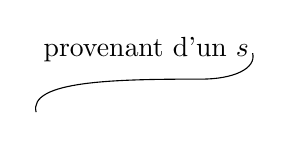
\begin{tikzpicture}[x=1cm,y=1cm]\node at (0,.35) {provenant d'un $s$};\draw (-1.4,-.45) .. controls (-1.5,-.05) and (-.4,-.03) .. (.7,-.03) .. controls (1.1,-.03) and (1.4,.1) .. (1.35,.3);\end{tikzpicture}}} dedans). D'autre part, $G(s')_{\mathbf C}$ est muni de $i(s'):G_{m\,\mathbf C}\to G(s')_{\mathbf C}$, et \unsure{on|qu'on} obtient par conséquent
\[
\unsure{v_{\zeta}|v_1}(s')=u(s')_{\mathbf C}\circ\bigl(i(s')\mid\mu_2\bigr):\mu_{2\,\mathbf C}\longrightarrow G_{\mathbf C}^{\zeta(s')}
\]
\deleted{D'autre part,} Ceci posé, il faut que $\pi^{\zeta(s')}$ (polarisation de $G_{\mathbf R}^{\zeta(s')}$ déduite de $\pi$ sur $G$ par transport) soit celle définie par les $\mu_{2\,\mathbf C}$. Par conséquent, pour $s'$ variable de façon que $\zeta(s')$ reste constant, les polarisations \inserted{\figure{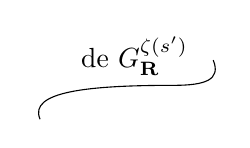
\begin{tikzpicture}[x=1cm,y=1cm]\node at (0,.35) {de $G_{\mathbf R}^{\zeta(s')}$};\draw (-1.2,-.45) .. controls (-1.35,-.1) and (-.6,-.02) .. (.5,-.02) .. controls (.9,-.02) and (1.1,.05) .. (1,.3);\end{tikzpicture}}} associées aux différents $v(s')$ doivent être identiques -- ce qui donne une condition non tautologique sur la distribution des \deleted{\unsure{$v$}} $u(s')$. [Noter cependant que l'ens des \deleted{classes de} polarisations d'un gpe réel \inserted{$H$}, défini en termes d'hom $\mu_{2\,\mathbf C}\to H_{\mathbf C}$, \margin{? à vérifier} est \uline{fini}, [si $G$ est commutatif en tous cas !], donc la restriction n'est pas tellement draconienne.

Enfin, conformément aux conjectures de Tate magnifiées, La connaissance des $u(s')$ permet de retrouver la structure d'effectivité dans la catégorie
\margin{184}
